\begin{tcolorbox}[colback=red!3!white,colframe=red!50!black,boxrule=0.8pt,title={Korrekturhinweise},fonttitle=\bfseries]
\textbf{Hinweis zum Stand Myon $g-2$ (2025).} Dieses Dokument bezieht sich auf die Abweichung zwischen gemessenem $a_\mu$ und der Standardmodell-Vorhersage, wie sie 2021 vorlag. Mit dem Fermilab-Endergebnis und dem White Paper~2025 der Muon~$g-2$ Theory Initiative ist diese Abweichung nicht mehr signifikant. Aussagen, die die Anomalie als Beleg oder als Zielgröße eines T0-Beitrags verwenden, sind überholt; den aktuellen Stand und die Einordnung gibt Dok.~382.

\textbf{Korrekturen aus der Rechenprüfung (30.~Sept.~2026)}, jeweils mit datiertem Vermerk an der Stelle:
\begin{itemize}
\item Schleifenintegral: fehlender Faktor $m_\ell^2$ ergänzt; der Abschnitt \enquote{vollständiges Integral} ($5/12$) entfällt, im Grenzfall $m_T \gg m_\ell$ gilt $2/3$. Endformel $\Delta a_\ell = \xi^4 m_\ell^2/(12\pi^2\lambda^2)$ statt $5\xi^4 m_\ell^2/(96\pi^2\lambda^2)$. Dimensionslos nur mit $\lambda$ als Masse (R91) und dimensionslos wirkender Kopplung $\xi$.
\item Normierungskonstante: $2{,}246 \times 10^{-13} \to 1{,}79 \times 10^{-56}$~GeV$^{-2}$ ($\lambda = m_P$); der alte Wert folgt aus keinem der genannten Parameter.
\item \enquote{Umrechnung in konventionelle Einheiten} (Faktor $10^6$) entfällt: $a_\ell$ ist dimensionslos. Damit $\Delta a_\mu \approx 2 \times 10^{-58}$ statt $251 \times 10^{-11}$ -- nicht messbar.
\item Die Entsprechung zu Dok.~018 und die \enquote{$\sim$2\,\% Präzision} beider Formulierungen treffen nicht zu; Hierarchie-Abschätzung um $\lambda^2$ ergänzt.
\end{itemize}
\end{tcolorbox}

\section*{Abstract}
		Dieses Dokument präsentiert die vollständige Lagrangian-Formulierung der T0-Theorie basierend auf dem fundamentalen geometrischen Parameter $\xi = \frac{4}{3} \times 10^{-4}$. Die Theorie etabliert eine fundamentale Zeit-Masse-Dualität $T(x,t) \cdot m(x,t) = 1$ und entwickelt einen erweiterten Lagrangian mit massenproportionaler Kopplung an ein dynamisches Zeitfeld. Für die geometrische Herleitung der anomalen magnetischen Momente und experimentelle Vorhersagen siehe Dokument 018\_T0\_Anomale-g2-10\_De.tex. Der Fokus liegt hier auf der feldtheoretischen Struktur und der Ableitung der fundamentalen T0-Beitragsformel aus ersten Prinzipien.

	
	
	\section{Einführung}
	
	\subsection{Grundprinzipien der T0-Theorie}
	
	Die T0-Theorie postuliert eine fundamentale Dualität zwischen Zeit und Masse:
	\begin{equation}
		T(x,t) \cdot m(x,t) = 1
		\label{eq:time_mass_duality}
	\end{equation}
	
	Diese Dualität führt zu mehreren fundamentalen Konsequenzen:
	\begin{itemize}
		\item Natürliche Massenhierarchie durch Zeitskalen
		\item Dynamische Massenerzeugung durch das Zeitfeld
		\item Quadratische Skalierung der anomalen magnetischen Momente mit $m_\ell^2$
		\item Intrinsische Integration der Gravitation in die Quantenfeldtheorie
	\end{itemize}
	
	\subsection{Der fundamentale geometrische Parameter}
	
	Die gesamte T0-Theorie basiert auf einem einzigen fundamentalen Parameter:
	\begin{equation}
		\boxed{\xi = \frac{4}{3} \times 10^{-4} = 1{,}333 \times 10^{-4}}
		\label{eq:xi_fundamental}
	\end{equation}
	
	Dieser dimensionslose Parameter kodiert die fundamentale geometrische Struktur des dreidimensionalen Raums. Für die detaillierte geometrische Interpretation und Herleitung siehe \href{https://github.com/jpascher/T0-Time-Mass-Duality/blob/main/2/pdf/018_T0_Anomale-g2-10_De.pdf}{Dokument 018}.
	
	\subsection{Notation und Konventionen}
	
	Wir verwenden natürliche Einheiten ($\hbar = c = 1$) mit Metriksignatur $(+,-,-,-)$:
	
	\begin{itemize}
		\item $T(x,t)$: Dynamisches Zeitfeld mit $[T] = E^{-1}$
		\item $\delta E(x,t)$: Fundamentales Energiefeld mit $[\delta E] = E$
		\item $\Delta m(x,t) = \delta E(x,t)$: Massenfeldfluktuationen
		\item $\xi = 1{,}333 \times 10^{-4}$: Fundamentaler geometrischer Parameter
		\item $\lambda$: Basismasse des Sektors (Nachtrag R91; im fundamentalen Sektor $m_P$)
		\item $m_\ell$: Leptonenmassen ($e$, $\mu$, $\tau$)
	\end{itemize}
	
	\subsection{Abgeleitete Parameter}
	
	Aus dem fundamentalen Parameter $\xi$ ergeben sich:
	\begin{align}
		\xi^2 &= \left(1{,}333 \times 10^{-4}\right)^2 = 1{,}777 \times 10^{-8} \label{eq:xi_squared} \\
		\xi^4 &= \left(1{,}333 \times 10^{-4}\right)^4 = 3{,}160 \times 10^{-16} \label{eq:xi_fourth}
	\end{align}
	
	\section{Erweiterter Lagrangian mit Zeitfeld}
	
	\subsection{Standardmodell-Lagrangian als Ausgangspunkt}
	
	Der Standardmodell-Lagrangian für ein Lepton $\psi_\ell$ lautet:
	\begin{equation}
		\mathcal{L}_{\text{SM}} = -\frac{1}{4} F_{\mu\nu}F^{\mu\nu} + \bar{\psi}_\ell(i\gamma^\mu D_\mu - m_\ell)\psi_\ell
		\label{eq:sm_lagrangian}
	\end{equation}
	
	Dabei ist:
	\begin{itemize}
		\item $F_{\mu\nu} = \partial_\mu A_\nu - \partial_\nu A_\mu$: Elektromagnetischer Feldstärketensor
		\item $D_\mu = \partial_\mu + ie A_\mu$: Kovariante Ableitung
		\item $m_\ell$: Leptonmasse (konstant)
	\end{itemize}
	
	\subsection{Einführung des dynamischen Zeitfeldes}
	
	In der T0-Theorie ist die Masse nicht konstant, sondern über die Zeit-Masse-Dualität \eqref{eq:time_mass_duality} an ein dynamisches Zeitfeld $T(x,t)$ gekoppelt. Wir führen das Massenfeld ein:
	\begin{equation}
		m(x,t) = m_0 + \Delta m(x,t)
		\label{eq:mass_field}
	\end{equation}
	
	wobei $m_0$ die Ruhemasse und $\Delta m(x,t)$ die dynamische Massenfluktuationen darstellt.
	
	\subsection{Kinetischer Term des Zeitfeldes}
	
	Das Zeitfeld selbst benötigt einen kinetischen Term:
	\begin{equation}
		\mathcal{L}_{\text{kin}}^{(T)} = \frac{1}{2}(\partial_\mu \Delta m)(\partial^\mu \Delta m)
		\label{eq:time_field_kinetic}
	\end{equation}
	
	Dieser Term beschreibt die Ausbreitung von Massenfeldfluktuationen als dynamische Freiheitsgrade.
	
	\subsection{Massenterm des Zeitfeldes}
	
	Das Zeitfeld hat eine charakteristische Masse $m_T$:
	\begin{equation}
		\mathcal{L}_{\text{mass}}^{(T)} = -\frac{1}{2} m_T^2 \Delta m^2
		\label{eq:time_field_mass}
	\end{equation}
	
	Die Zeitfeldmasse $m_T$ ist über die Higgs-Zeitfeld-Verbindung gegeben durch:
	\begin{equation}
		m_T = \frac{\lambda}{\xi}
		\label{eq:time_field_mass_value}
	\end{equation}
	
	wobei $\lambda$ die Basismasse des jeweiligen Sektors ist (im fundamentalen Sektor $m_P$). \textit{(Korrigiert am 30.~Sept.~2026: vorher \enquote{Higgs-Kopplungsparameter} -- dimensional muss $\lambda$ eine Masse sein, siehe Nachtrag R91.)}
	
	\subsection{Massenproportionale Kopplung}
	
	Der fundamentale neue Term in der T0-Theorie ist die Kopplung der Leptonfelder an das Zeitfeld, proportional zur Leptonmasse:
	\begin{equation}
		\mathcal{L}_{\text{int}} = g_T^\ell \, \bar{\psi}_\ell \psi_\ell \, \Delta m
		\label{eq:interaction_term}
	\end{equation}
	
	Die Kopplungsstärke ist gegeben durch:
	\begin{equation}
		\boxed{g_T^\ell = \xi \, m_\ell}
		\label{eq:coupling_strength}
	\end{equation}
	
	Diese massenproportionale Kopplung ist das Herzstück der T0-Theorie. Sie impliziert:
	\begin{itemize}
		\item Schwerere Leptonen koppeln stärker an das Zeitfeld
		\item Die Kopplung skaliert linear mit der Masse
		\item Dies führt zu quadratischer Massenskalierung in Quantenkorrekturen
	\end{itemize}
	
	\subsection{Vollständiger erweiterter Lagrangian}
	
	Der vollständige T0-Lagrangian kombiniert alle Terme:
	\begin{equation}
		\begin{split}
			\mathcal{L}_{\text{T0}} = &-\frac{1}{4} F_{\mu\nu}F^{\mu\nu} \\
			&+ \bar{\psi}_\ell(i\gamma^\mu D_\mu - m_\ell)\psi_\ell \\
			&+ \frac{1}{2}(\partial_\mu \Delta m)(\partial^\mu \Delta m) \\
			&- \frac{1}{2} m_T^2 \Delta m^2 \\
			&+ \xi \, m_\ell \,\bar{\psi}_\ell \psi_\ell \, \Delta m
		\end{split}
		\label{eq:full_lagrangian}
	\end{equation}
	
	\section{Quantenkorrekturen und Feynman-Regeln}
	
	\subsection{Feynman-Regeln aus dem Lagrangian}
	
	Aus dem Wechselwirkungsterm \eqref{eq:interaction_term} ergeben sich die Feynman-Regeln:
	
	\textbf{Vertex-Faktor:}
	\begin{equation}
		\bar{\psi}_\ell \psi_\ell \Delta m \quad \longrightarrow \quad -i g_T^\ell = -i \xi m_\ell
		\label{eq:vertex_factor}
	\end{equation}
	
	\textbf{Zeitfeld-Propagator:}
	\begin{equation}
		\Delta m(k) \quad \longrightarrow \quad \frac{i}{k^2 - m_T^2 + i\epsilon}
		\label{eq:propagator}
	\end{equation}
	
	\subsection{Ein-Schleifen-Diagramm}
	
	Das fundamentale Ein-Schleifen-Diagramm für den anomalen magnetischen Moment-Beitrag hat die Struktur:
\begin{center}
	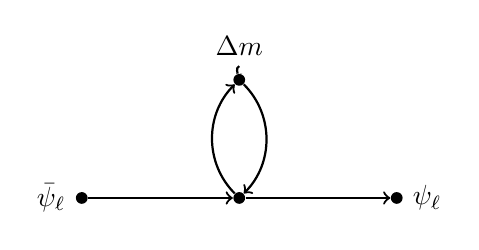
\begin{tikzpicture}[
		vertex/.style={circle,fill,inner sep=1.5pt},
		fermion/.style={->,thick},
		scalar/.style={dashed,thick}
		]
		% Vertices
		\node[vertex,label=left:$\bar{\psi}_\ell$] (a) at (0,0) {};
		\node[vertex] (b) at (2,0) {};
		\node[vertex,label=right:$\psi_\ell$] (c) at (4,0) {};
		\node[vertex] (d) at (2,1.5) {};
		
		% Lines
		\draw[fermion] (a) -- (b);
		\draw[fermion] (b) -- (c);
		\draw[fermion] (b) to[bend left=45] (d);
		\draw[fermion] (d) to[bend left=45] (b);
		\draw[scalar] (d) to[loop above,looseness=8] node[above] {$\Delta m$} (d);
	\end{tikzpicture}
\end{center}


	
	\subsection{Allgemeine Formel für skalare Mediatoren}
	
	Für einen skalaren Mediator mit Masse $m_T$ und Kopplung $g_T^\ell$ lautet die allgemeine Ein-Schleifen-Formel:
	\begin{equation}
		\begin{split}
			\Delta a_\ell = \frac{(g_T^\ell)^2}{8\pi^2} \int_0^1 dx \, 
			\frac{m_\ell^2 (1-x)(1-x^2)}{m_\ell^2 x^2 + m_T^2 (1-x)}
		\end{split}
		\label{eq:general_loop_formula}
	\end{equation}
	
	Diese Formel ist Standard in der Quantenfeldtheorie für skalare Beiträge zum anomalen magnetischen Moment.
	
	\section{Ableitung der fundamentalen T0-Formel}
	
	\subsection{Grenzfall schwerer Mediatoren}
	
	Für $m_T \gg m_\ell$ kann das Integral \eqref{eq:general_loop_formula} vereinfacht werden. Im Nenner dominiert der Term $m_T^2 (1-x)$:
	\begin{equation}
		\frac{m_\ell^2 (1-x)(1-x^2)}{m_\ell^2 x^2 + m_T^2 (1-x)} 
		\approx \frac{m_\ell^2 (1-x)(1-x^2)}{m_T^2 (1-x)} 
		= \frac{m_\ell^2 (1-x^2)}{m_T^2}
		\label{eq:heavy_mediator_approx}
	\end{equation}
	
	Damit wird:
	\begin{equation}
		\begin{split}
			\Delta a_\ell &\approx \frac{(g_T^\ell)^2 m_\ell^2}{8\pi^2 m_T^2} \int_0^1 dx \, (1-x^2) \\
			&= \frac{(g_T^\ell)^2 m_\ell^2}{8\pi^2 m_T^2} \left[x - \frac{x^3}{3}\right]_0^1 \\
			&= \frac{(g_T^\ell)^2 m_\ell^2}{8\pi^2 m_T^2} \left(1 - \frac{1}{3}\right) \\
			&= \frac{(g_T^\ell)^2 m_\ell^2}{8\pi^2 m_T^2} \cdot \frac{2}{3}
		\end{split}
		\label{eq:integral_evaluation}
	\end{equation}
	\textit{(Korrigiert am 30.~Sept.~2026: vorher ohne den Faktor $m_\ell^2$ -- er steht in Gl.~\eqref{eq:heavy_mediator_approx} und darf beim Herausziehen vor das Integral nicht verloren gehen.)}
	
	\subsection{Einsetzen der T0-Kopplung}
	
	Mit der massenproportionalen Kopplung \eqref{eq:coupling_strength} erhalten wir:
	\begin{equation}
		\begin{split}
			\Delta a_\ell &= \frac{\xi^2 m_\ell^2}{8\pi^2 m_T^2} \cdot \frac{2}{3} \\
			&= \frac{2 \xi^2 m_\ell^2}{24\pi^2 m_T^2} \\
			&= \frac{\xi^2 m_\ell^2}{12\pi^2 m_T^2}
		\end{split}
		\label{eq:t0_coupling_inserted}
	\end{equation}
	\textit{(Korrigiert am 30.~Sept.~2026: vorher erste Zeile $(\xi m_\ell)^2/(8\pi^2 m_T^2)\cdot 2/3$ -- dort ersetzte die Kopplung $\xi m_\ell$ den in Gl.~\eqref{eq:integral_evaluation} verlorenen Faktor $m_\ell^2$. Mit $m_\ell^2$ aus dem Schleifenintegral ist das Ergebnis nur dann dimensionslos und quadratisch in $m_\ell$, wenn die Kopplung im Wechselwirkungsterm als dimensionsloses $\xi$ wirkt; $g_T^\ell = \xi m_\ell$ hätte die Dimension einer Masse und ergäbe $m_\ell^4$ mit $[\Delta a] = E^2$. Die Massenproportionalität steckt damit im Faktor $m_\ell^2$ der Schleife. Das Ergebnis dieser Zeile ist unverändert.)}
	
	\subsection{Higgs-Zeitfeld-Verbindung}
	
	Mit der Zeitfeldmasse \eqref{eq:time_field_mass_value} wird:
	\begin{equation}
		\begin{split}
			\Delta a_\ell &= \frac{\xi^2 m_\ell^2}{12\pi^2 (\lambda/\xi)^2} \\
			&= \frac{\xi^2 m_\ell^2}{12\pi^2} \cdot \frac{\xi^2}{\lambda^2} \\
			&= \frac{\xi^4 m_\ell^2}{12\pi^2 \lambda^2}
		\end{split}
		\label{eq:higgs_connection_substituted}
	\end{equation}
	
	\subsection{Endformel}

	Gl.~\eqref{eq:higgs_connection_substituted} ist bereits die Endformel des Grenzfalls $m_T \gg m_\ell$:
	\begin{equation}
		\boxed{\Delta a_\ell^{\text{(T0)}} = \frac{\xi^4}{12\pi^2\lambda^2} \cdot m_\ell^2}
		\label{eq:t0_fundamental_formula}
	\end{equation}
	\textit{(Korrigiert am 30.~Sept.~2026: vorher Abschnitt \enquote{Korrektur durch vollständiges Integral} mit $\int_0^1(1-x)(1-x^2)\,dx = 5/12$ und Endformel $5\xi^4 m_\ell^2/(96\pi^2\lambda^2)$ -- im Grenzfall $m_T \gg m_\ell$ kürzt sich $(1-x)$ gegen den Nenner (Gl.~\eqref{eq:heavy_mediator_approx}); das Integral ist $\int_0^1(1-x^2)\,dx = 2/3$, wie oben gerechnet. $5/12$ wäre der Zähler ohne den Nenner.)}

	Dimensionslos ist $\Delta a_\ell$ genau dann, wenn $\lambda$ eine Masse ist -- das ist die Lesart des Nachtrags R91: $\lambda = M_\text{Basis}$, im fundamentalen Sektor $M_\text{Basis} = m_P$.

	\section{Numerische Auswertung}

	\subsection{Bestimmung der Normierungskonstante}

	Die Normierungskonstante lautet:
	\begin{equation}
		C_{\text{T0}} = \frac{\xi^4}{12\pi^2\lambda^2}
		\label{eq:normalization_constant}
	\end{equation}

	Mit $\xi^4 = 3{,}160 \times 10^{-16}$ und $\lambda = m_P = 1{,}221 \times 10^{19}$~GeV (Nachtrag R91) erhalten wir:
	\begin{equation}
		C_{\text{T0}} = \frac{3{,}160 \times 10^{-16}}{118{,}4 \times 1{,}491 \times 10^{38}\ \text{GeV}^2} = 1{,}79 \times 10^{-56} \text{ GeV}^{-2}
		\label{eq:numerical_constant}
	\end{equation}
	\textit{(Korrigiert am 30.~Sept.~2026: vorher $C_\text{T0} \approx 2{,}246 \times 10^{-13}$~GeV$^{-2}$, angeblich aus $\lambda_h \approx 0{,}13$, $v$, $m_h$ und $\xi = \lambda_h^2 v^2/(16\pi^3 m_h^2)$ -- dieser Wert folgt aus keinem der genannten Parameter: mit $\lambda = 0{,}13$ ergäbe die Formel $1{,}6 \times 10^{-16}$ (dimensionslos), $2{,}246 \times 10^{-13}$~GeV$^{-2}$ verlangte $\lambda = 2{,}7$~MeV. Die Relation $\xi = \lambda_h^2 v^2/(16\pi^3 m_h^2) = 1{,}32 \times 10^{-4}$ ist davon unabhängig.)}

	\subsection{Finale T0-Beitragsformel}

	Die vollständig ausgewertete T0-Beitragsformel lautet:
	\begin{equation}
		\boxed{\Delta a_\ell^{\text{(T0)}} = 1{,}79 \times 10^{-56} \cdot m_\ell^2 \text{ [GeV}^{-2}\text{]}}
		\label{eq:final_t0_formula}
	\end{equation}

	wobei $m_\ell$ in GeV einzusetzen ist.

	\subsection{Leptonspezifische Vorhersagen}

	Mit den Leptonmassen:
	\begin{itemize}
		\item $m_e = 0{,}511$ MeV $= 0{,}000511$ GeV
		\item $m_\mu = 105{,}658$ MeV $= 0{,}105658$ GeV
		\item $m_\tau = 1776{,}86$ MeV $= 1{,}77686$ GeV
	\end{itemize}

	ergeben sich die T0-Beiträge:

	\textbf{Elektron:}
	\begin{equation}
		\begin{split}
			\Delta a_e^{\text{(T0)}} &= 1{,}79 \times 10^{-56} \cdot (0{,}000511)^2 \\
			&= 1{,}79 \times 10^{-56} \cdot 2{,}611 \times 10^{-7} \\
			&= 4{,}7 \times 10^{-63}
		\end{split}
		\label{eq:electron_prediction}
	\end{equation}

	\textbf{Myon:}
	\begin{equation}
		\begin{split}
			\Delta a_\mu^{\text{(T0)}} &= 1{,}79 \times 10^{-56} \cdot (0{,}105658)^2 \\
			&= 1{,}79 \times 10^{-56} \cdot 1{,}1164 \times 10^{-2} \\
			&= 2{,}0 \times 10^{-58}
		\end{split}
		\label{eq:muon_prediction}
	\end{equation}

	\textbf{Tau:}
	\begin{equation}
		\begin{split}
			\Delta a_\tau^{\text{(T0)}} &= 1{,}79 \times 10^{-56} \cdot (1{,}77686)^2 \\
			&= 1{,}79 \times 10^{-56} \cdot 3{,}1572 \\
			&= 5{,}7 \times 10^{-56}
		\end{split}
		\label{eq:tau_prediction}
	\end{equation}
	\textit{(Korrigiert am 30.~Sept.~2026: vorher mit $C_\text{T0} = 2{,}246 \times 10^{-13}$ die Werte $5{,}86 \times 10^{-20}$, $2{,}51 \times 10^{-15}$ und $7{,}09 \times 10^{-13}$.)}

	\subsection{Keine Umrechnung nötig}

	Das anomale magnetische Moment $a_\ell = (g_\ell - 2)/2$ ist dimensionslos; die obigen Werte sind bereits die Werte, die mit dem Experiment zu vergleichen sind (oft angegeben in Einheiten von $10^{-11}$). Der Lagrange-Beitrag des Zeitfelds ist damit um viele Größenordnungen kleiner als jede Messgenauigkeit.

	\textit{(Korrigiert am 30.~Sept.~2026: vorher Abschnitt \enquote{Umrechnung in konventionelle Einheiten}, der alle Werte mit $10^6$ multiplizierte: $\Delta a_\mu = 2{,}51 \times 10^{-9} = 251 \times 10^{-11}$, $\Delta a_e = 5{,}86 \times 10^{-14}$, $\Delta a_\tau = 7{,}09 \times 10^{-7}$ -- eine dimensionslose Größe ändert sich bei einer Umrechnung nicht, auch ein Wechsel MeV/GeV ergibt keinen Faktor. $251 \times 10^{-11}$ war die Myon-Anomalie des Stands 2021; Konstante und Faktor ergaben diesen Wert nur zusammen. Die Anomalie ist seit 2025 nicht mehr signifikant (Dok.~382), ein vernachlässigbarer Lagrange-Beitrag steht dazu nicht im Widerspruch.)}

	\section{Quadratische Massenskalierung}
	
	\subsection{Fundamentale Vorhersage}
	
	Die zentrale Vorhersage der T0-Theorie ist die quadratische Massenskalierung \eqref{eq:final_t0_formula}:
	\begin{equation}
		\Delta a_\ell^{\text{(T0)}} \propto m_\ell^2
		\label{eq:quadratic_scaling}
	\end{equation}
	
	Dies führt zu natürlichen Hierarchien:
	\begin{align}
		\frac{\Delta a_e^{\text{(T0)}}}{\Delta a_\mu^{\text{(T0)}}} 
		&= \left(\frac{m_e}{m_\mu}\right)^2 
		= \left(\frac{0{,}511}{105{,}658}\right)^2 
		= 2{,}34 \times 10^{-5} \label{eq:electron_muon_ratio} \\
		\frac{\Delta a_\tau^{\text{(T0)}}}{\Delta a_\mu^{\text{(T0)}}} 
		&= \left(\frac{m_\tau}{m_\mu}\right)^2 
		= \left(\frac{1776{,}86}{105{,}658}\right)^2 
		= 282{,}8 \label{eq:tau_muon_ratio}
	\end{align}
	
	\subsection{Physikalische Interpretation}
	
	Die quadratische Massenskalierung hat tiefe physikalische Bedeutung:
	
	\textbf{Ursache:} Die Kopplung ist massenproportional $g_T^\ell = \xi m_\ell$. Im Ein-Schleifen-Beitrag erscheint $(g_T^\ell)^2 = \xi^2 m_\ell^2$.
	
	\textbf{Konsequenzen:}
	\begin{itemize}
		\item Elektron-Effekte sind relativ zum Myon um $\sim 10^{-5}$ kleiner
		\item Myon-Effekte liegen bei $\sim 10^{-58}$ und sind nicht messbar
		\item Tau-Effekte sind relativ am größten ($\sim 280 \times$ größer als Myon), absolut ebenfalls vernachlässigbar
	\end{itemize}
	\textit{(Korrigiert am 30.~Sept.~2026: vorher \enquote{Myon-Effekte sind messbar ($\sim 10^{-9}$)} und \enquote{Tau-Effekte sind dominant} -- Folge des Faktors $10^6$ und der Konstante $2{,}246 \times 10^{-13}$; die Verhältnisse $2{,}34 \times 10^{-5}$ und $282{,}8$ bleiben gültig.)}
	
	\textbf{Vergleich mit QED:} In der Standardtheorie skaliert der führende Beitrag wie $\alpha/(2\pi)$, unabhängig von der Masse. Die T0-Theorie fügt einen massenabhängigen Beitrag hinzu.
	
	\section{Verbindung zur geometrischen Formulierung}
	
	\subsection{Verhältnis zur g-2 Analyse}
	
	Die hier abgeleiteten T0-Beiträge $\Delta a_\ell^{\text{(T0)}}$ sind zusätzliche Beiträge zum Standardmodell. Sie sind \textbf{nicht} dieselben Größen wie die in Dokument 018 geometrisch hergeleiteten Werte: Dok.~018 erhält $\Delta a(\mu{-}e) = 4{,}37 \times 10^{-6}$ aus $4\pi/f^{p}$, hier ergibt sich ein Beitrag $\propto m_\ell^2$ von $\sim 10^{-58}$. Die tragende g-2-Linie ist die Verhältnis-Linie in Dok.~018 und 158. \textit{(Korrigiert am 30.~Sept.~2026: vorher \enquote{Sie entsprechen den in Dokument 018 geometrisch hergeleiteten Werten} -- die beiden Formulierungen liefern um viele Größenordnungen verschiedene Beiträge mit verschiedener Massenabhängigkeit.)}
	
	Der Unterschied in der Notation:
	\begin{itemize}
		\item \textbf{Dokument 018:} Berechnet direkt $a_\ell$ (inklusive SM + T0)
		\item \textbf{Dieses Dokument:} Berechnet $\Delta a_\ell^{\text{(T0)}}$ (nur T0-Beitrag)
	\end{itemize}
	
	Die Relation ist:
	\begin{equation}
		a_\ell^{\text{(total)}} = a_\ell^{\text{(SM)}} + \Delta a_\ell^{\text{(T0)}}
		\label{eq:total_relation}
	\end{equation}
	
	\subsection{Parameter-Entsprechungen}
	
	Die geometrischen Parameter aus Dokument 018 entsprechen den Lagrangian-Parametern:
	\begin{align}
		\xi &= \frac{4}{3} \times 10^{-4} \quad \text{(identisch in beiden Formulierungen)} \label{eq:xi_correspondence} \\
		f &= 7500 \quad \text{(geometrischer Sub-Planck-Faktor)} \label{eq:f_correspondence} \\
		\varphi &= \frac{1+\sqrt{5}}{2} \quad \text{(pentagonale Symmetriebrechung)} \label{eq:phi_correspondence}
	\end{align}
	
	Gemeinsam ist beiden Formulierungen der Parameter $\xi$; eine zahlenmäßige Verbindung der Beiträge besteht nicht (siehe oben). Der Projektionsfaktor $k_{\text{geom}}$ gehört allein zur geometrischen 4D-3D-Projektion in Dok.~018.
	
	\section{Higgs-Mechanismus in der T0-Theorie}
	
	\subsection{Higgs-Feld als fundamentale Basis}
	
	In der T0-Theorie ist das Higgs-Feld nicht ein zusätzliches Feld, sondern die fundamentale Basis der Zeit-Masse-Dualität:
	\begin{equation}
		T(x,t) \cdot m(x,t) = 1
		\label{eq:higgs_foundation}
	\end{equation}
	
	Der universelle Parameter $\xi$ folgt direkt aus den Higgs-Parametern:
	\begin{equation}
		\boxed{\xi = \frac{\lambda_h^2 v^2}{16\pi^3 m_h^2}}
		\label{eq:xi_from_higgs}
	\end{equation}
	
	mit:
	\begin{itemize}
		\item $\lambda_h$: Higgs-Selbstkopplung
		\item $v = 246$ GeV: Higgs-Vakuumerwartungswert
		\item $m_h = 125$ GeV: Higgs-Masse
	\end{itemize}
	
	\subsection{Spontane Symmetriebrechung}
	
	Die spontane Symmetriebrechung des Higgs-Feldes erzeugt:
	\begin{itemize}
		\item Leptonmassen durch Yukawa-Kopplung
		\item Das Zeitfeld $T(x,t)$ als Fluktuationen um den VEV
		\item Die Zeit-Masse-Dualität als fundamentale Struktur
	\end{itemize}
	
	In diesem Bild sind Massenfluktuationen $\Delta m$ direkt mit Higgs-Fluktuationen verbunden:
	\begin{equation}
		\Delta m(x,t) = y_\ell \cdot \delta h(x,t)
		\label{eq:higgs_fluctuation}
	\end{equation}
	
	wobei $y_\ell$ die Yukawa-Kopplung und $\delta h$ die Higgs-Fluktuation ist.
	
	\section{Feldtheoretische Struktur}
	
	\subsection{Bewegungsgleichungen}
	
	Aus dem Lagrangian \eqref{eq:full_lagrangian} folgen die Euler-Lagrange-Gleichungen:
	
	\textbf{Für das Leptonfeld:}
	\begin{equation}
		(i\gamma^\mu D_\mu - m_\ell - \xi m_\ell \Delta m)\psi_\ell = 0
		\label{eq:lepton_eom}
	\end{equation}
	
	\textbf{Für das Zeitfeld:}
	\begin{equation}
		\Box \Delta m + m_T^2 \Delta m = \xi m_\ell \bar{\psi}_\ell \psi_\ell
		\label{eq:time_field_eom}
	\end{equation}
	
	wobei $\Box = \partial_\mu \partial^\mu$ der d'Alembert-Operator ist.
	
	\subsection{Interpretation der Bewegungsgleichungen}
	
	Gleichung \eqref{eq:lepton_eom} zeigt, dass das Lepton eine effektive Masse hat:
	\begin{equation}
		m_{\text{eff}}(x,t) = m_\ell (1 + \xi \Delta m)
		\label{eq:effective_mass}
	\end{equation}
	
	Die Masse wird durch das Zeitfeld moduliert.
	
	Gleichung \eqref{eq:time_field_eom} zeigt, dass das Zeitfeld eine Quelle hat:
	\begin{equation}
		\text{Quelle} = \xi m_\ell \bar{\psi}_\ell \psi_\ell = \xi m_\ell \rho_\ell
		\label{eq:source_term}
	\end{equation}
	
	Die Leptondichte $\rho_\ell$ erzeugt Zeitfeldfluktuationen, proportional zur Leptonmasse.
	
	\subsection{Energieskalen}
	
	Die charakteristischen Energieskalen in der Theorie sind:
	\begin{align}
		E_{\text{Lepton}} &\sim m_\ell \quad \text{(Leptonmasse)} \label{eq:lepton_scale} \\
		E_{\text{Zeit}} &\sim m_T = \frac{\lambda}{\xi} \quad \text{(Zeitfeldmasse)} \label{eq:time_scale} \\
		E_{\text{Kopplung}} &\sim \xi m_\ell \ll m_\ell \quad \text{(schwache Kopplung)} \label{eq:coupling_scale}
	\end{align}
	
	Die Hierarchie $E_{\text{Kopplung}} \ll E_{\text{Lepton}} \ll E_{\text{Zeit}}$ rechtfertigt die störungstheoretische Behandlung.
	
	\section{Renormierung (historische Darstellung)}

\textbf{Hinweis:} Dieser Abschnitt verwendet die Sprache der QFT-Renormierung (Wellenfunction-Renormierung, $\beta$-Funktion, RG-Gleichungen) als Beschreibungsmittel. In der vollständigen FFGFT-Formulierung (Dok.~202) ist traditionelle Renormierung nicht erforderlich: der fraktale Torus liefert einen natürlichen UV-Cutoff bei $E_P/\xi$, und die Skalenstruktur folgt aus der Rekursion $\mathcal{R}$. Die hier verwendeten Formeln sind mit der FFGFT-Struktur kompatibel, aber die Terminologie ist näher am SM als an der nativen FFGFT-Sprache.
	
	\subsection{Divergenzen in Schleifendiagrammen}
	
	Das Ein-Schleifen-Integral \eqref{eq:general_loop_formula} ist für $m_T \gg m_\ell$ endlich. Höhere Ordnungen können jedoch Divergenzen enthalten.
	
	Die Renormierung der T0-Theorie erfordert:
	\begin{itemize}
		\item Wellenfunction-Renormierung für $\psi_\ell$ und $\Delta m$
		\item Massen-Renormierung für $m_\ell$ und $m_T$
		\item Kopplungs-Renormierung für $g_T^\ell$
	\end{itemize}
	
	\subsection{Renormierungsgruppen-Gleichungen}
	
	Die Laufende Kopplung folgt:
	\begin{equation}
		\mu \frac{d g_T^\ell}{d\mu} = \beta_{g_T}(g_T^\ell)
		\label{eq:rg_equation}
	\end{equation}
	
	Aufgrund der massenproportionalen Struktur \eqref{eq:coupling_strength} ist:
	\begin{equation}
		\beta_{g_T} = \xi \beta_m
		\label{eq:beta_relation}
	\end{equation}
	
	wobei $\beta_m$ die anomale Massendimension ist.
	
	\subsection{Konsistenz mit Standardmodell}
	
	Die T0-Beiträge sind subdominant gegenüber den Standardmodell-Beiträgen:
	\begin{equation}
		\frac{\Delta a_\ell^{\text{(T0)}}}{a_\ell^{\text{(QED)}}} \sim \frac{\xi^4 m_\ell^2}{6\pi\alpha\lambda^2} \ll 1
		\label{eq:hierarchy}
	\end{equation}
	
	\textit{(Korrigiert am 30.~Sept.~2026: vorher $\xi^4 m_\ell^2/\alpha$ -- ohne $\lambda^2$ nicht dimensionslos; mit $a^\text{(QED)} \approx \alpha/(2\pi)$ und Gl.~\eqref{eq:t0_fundamental_formula} folgt der obige Ausdruck.)}

	Dies garantiert Konsistenz mit experimentellen Daten und ermöglicht störungstheoretische Behandlung.
	
	\section{Vergleich verschiedener Formulierungen}
	
	\subsection{Lagrangian vs. geometrische Formulierung}
	
	\begin{table}[h]
		\centering
		\adjustbox{max width=\textwidth}{%
\begin{tabular}{lcc}
			\toprule
			\textbf{Aspekt} & \textbf{Lagrangian (Dok. 019)} & \textbf{Geometrisch (Dok. 018)} \\
			\midrule
			Ausgangspunkt & Zeitfeld $\Delta m(x,t)$ & Torsionsgitter, Windungen \\
			Methode & Feldtheorie, Schleifenintegrale & Fraktale Geometrie \\
			Hauptformel & $\Delta a \propto \xi^4 m^2$ & $a \propto f \xi m^{p}$ \\
			Vorhersage & T0-Beitrag $\Delta a$ & Gesamtwert $a$ \\
			Parameter & $\xi$, $\lambda$, $m_T$ & $\xi$, $\varphi$, $f$ \\
			\bottomrule
		\end{tabular}%
}
		\caption{Vergleich der Formulierungen}
		\label{tab:comparison}
	\end{table}
	
	\subsection{Komplementarität}
	
	Die beiden Formulierungen sind komplementär:
	\begin{itemize}
		\item \textbf{Lagrangian:} Gibt die feldtheoretische Struktur und Feynman-Regeln
		\item \textbf{Geometrisch:} Gibt die physikalische Intuition und Verhältnis-Vorhersagen
	\end{itemize}
	
	Die numerischen Vorhersagen für $a_\ell$ stammen aus der geometrischen Formulierung (Dok.~018, 158); der Lagrange-Beitrag des Zeitfelds ist vernachlässigbar klein. \textit{(Korrigiert am 30.~Sept.~2026: vorher \enquote{Beide führen zu konsistenten numerischen Vorhersagen mit $\sim$2\,\% Präzision} -- siehe Abschnitt \enquote{Verhältnis zur g-2 Analyse}.)}
	
	\section*{Literaturverzeichnis}
	
	\begin{thebibliography}{99}
		
		\bibitem{t0_g2_2026}
		J. Pascher,
		\textit{Anomale magnetische Momente in der FFGFT-Theorie: Geometrische Herleitung aus der Zeit-Masse-Dualität},
		\href{https://github.com/jpascher/T0-Time-Mass-Duality/blob/main/2/pdf/018_T0_Anomale-g2-10_De.pdf}{Dokument 018\_T0\_Anomale-g2-10\_De.pdf},
		Februar 2026.
		
		\bibitem{peskin_schroeder_1995}
		M. E. Peskin, D. V. Schroeder,
		\textit{An Introduction to Quantum Field Theory},
		Westview Press, 1995.
		Standardreferenz für Feynman-Regeln und Schleifenberechnungen.
		
		\bibitem{pdg_2024}
		Particle Data Group,
		\textit{Review of Particle Physics},
		Prog. Theor. Exp. Phys. 2024, 083C01 (2024).
		Experimentelle Werte für Leptonmassen und g-2.
		
		\bibitem{higgs_1964}
		P. W. Higgs,
		\textit{Broken Symmetries and the Masses of Gauge Bosons},
		Phys. Rev. Lett. 13, 508 (1964).
		Original-Higgs-Mechanismus.
		
		\bibitem{weinberg_qft}
		S. Weinberg,
		\textit{The Quantum Theory of Fields, Volume I: Foundations},
		Cambridge University Press, 1995.
		Umfassende Behandlung der Quantenfeldtheorie.
		
	\end{thebibliography}
	
% ============================================================
% Nachtrag 7. September 2026 — R91: lambda in m_T = lambda/xi
% Quelle: Dok. 190-Archiv-2 (R91)
% Quelldokument bleibt unverändert (append-only, vgl. R50).
% ============================================================

\section*{Nachtrag R91: Beschriftungskorrektur $m_T = \lambda/\xi$ (7.~September 2026)}

Die Bezeichnung $\lambda$ als „Higgs-Kopplungsparameter" in der Formel
$m_T = \lambda/\xi$ ist \textbf{irreführend} (R91, Dok.~190-Archiv-2).

\textbf{Drei Gründe:}
(i)~Dimensional muss $\lambda$ eine \emph{Masse} sein, da $m_T$ eine Masse
und $\xi$ dimensionslos ist; der Higgs-Quartic $\lambda_h \approx 0{,}129$
ist hingegen dimensionslos.
(ii)~$\lambda_h$ läuft unter der RGE und ist ein Niederenergie-Parameter
der elektroschwachen Skala; ein dort gemessener Wert ist an der Planck-Skala
nicht einsetzbar.
(iii)~Als dimensionsloser Faktor in Planck-Einheiten interpretiert ergäbe
$\lambda_h$ die Reichweite $7{,}75\cdot L_0$ --- verfehlt $L_0$.

\textbf{Korrekt:} $\lambda = M_\text{Basis}$ ist die Basismasse des jeweiligen
Sektors; im fundamentalen Sektor $M_\text{Basis} = m_P$ (R89/R90, Dok.~180).
Die Formel lautet strukturell $m_T = M_\text{Basis}/\xi$, sektorabhängiger Wert,
universelle Form. Eine Higgs-Verbindung kann allenfalls eine effektive Aussage im
elektroschwachen Sektor sein, nie die Definition.
